\documentclass[draft, english]{jflart}
\usepackage[utf8]{inputenc}
\usepackage[T1]{fontenc}

% Numéro et année des JFLAs visées par l'article, obligatoire.
\jfla{35}{2024}

\title{Soumettre un article aux Journées Francophones des Langages Applicatifs\\
  en utilisant la classe~\texttt{jflart.cls}}
% Un titre plus court, optionnel.
\titlerunning{Du bon usage de~\texttt{jflart.cls}}

% Auteurs, liste non abrégée.
\author[1]{Eusèbe Tartempion}
\author[2]{Cunégonde Martin}
\author[2]{Odoacre Contempierre}
% Une liste d'auteurs abrégée à utiliser à l'intérieur de l'article.
\authorrunning{Tartempion, Martin et Contempierre}

% Affiliations des auteurs
\affil[1]{Université Paris Université, CNRS, INRIA, CEA, INRA, INSERM, Paris, 75013, France}
\affil[2]{Université Sorbonne Très Grand Sud, Nice, 06000, France}

% Une commande définie par l'utilisateur
\newcommand{\cmd}[1]{\texttt{\textbackslash {#1}}}

\begin{document}

\maketitle

\begin{abstract}
  Le résumé peut venir avant ou après la commande maketitle.
  %
  Il devrait contenir aussi peu de commandes LaTeX que possible pour faciliter
  la conversion vers HTML nécessaire à son inclusion dans les actes et sur le
  site web des JFLA.
\end{abstract}

\section{Introduction}

Les Journées Francophones des Langages Applicatifs~\cite{JFLA} sont organisées
par vos collègues de façon volontaire et bénévole.
%
L'objectif des présentes instructions est de simplifier le processus de
relecture des articles soumis et la publication des articles acceptés.

\section{Consignes générales}

Pour maintenir l'uniformité des actes des JFLA, nous vous demandons de ne
changer ni la police par défaut ni sa taille (10 points).
%
En particulier, l'usage de paquets comme~\texttt{times} ou~\texttt{libertine}
est interdit.
%
Modifier les paramètres typographiques qui régissent l'apparence du code
informatique ou des formules mathématiques pour faire tenir un contenu trop
dense dans une zone trop étroite est également de mauvais aloi.

L'usage des commandes de positionnement et d'espacement explicites,
notamment~\cmd{vspace} et ses cousines, doit être minimisé.
%
La commande~\cmd{sloppy} ne doit être utilisée qu'en ultime recours,
lorsqu'aucune reformulation du texte n'est possible.

L'option~\texttt{draft} doit impérativement être utilisée lors de la production
de la version soumise pour relecture.
%
Elle devra être remplacée par l'option~\texttt{final} pour la version finale.

\section{Options de la classe}

\paragraph{Option~\texttt{english}.}

La classe suppose par défaut un article rédigé en langue française.
%
Cette option est à utiliser si l'article est rédigé en langue anglaise.

\paragraph{Option~\texttt{draft}.}

Cette option rajoute les numéros de lignes dans la marge.

\paragraph{Option~\texttt{final}.}

L'option~\texttt{final} prépare l'article à l'inclusion dans les actes de la
conférence.

\section{Paquets chargés par défaut}

La classe~\texttt{jflart.cls} charge un certain nombre de paquets par défaut.
%
\begin{itemize}
\item
  %
  Le paquet~\texttt{babel} pour la prise en charge de la langue française ou
  anglaise.

\item
  %
  Les paquets~\texttt{color} et~\texttt{graphicx}, pour permettre l'usage de
  couleurs et l'inclusion d'images.

\item
  %
  Le paquet~\texttt{hyperref}, pour l'ajout des hyperliens.
  %
  Ceux-ci, par défaut, ne sont pas mis en surbrillance afin de préserver le gris
  typographique du texte.

\item
  %
  Les paquets de l'\emph{American Mathematical Society}, à
  savoir~\texttt{amsmath}, \texttt{amssymb} et~\texttt{amsthm}.
  %
  Nous recommandons vivement l'usage des environnements proposés par ces paquets
  pour énoncer théorèmes, lemmes et définitions (voir plus bas), ainsi que pour
  aligner d'éventuelles équations et
  formules~(environnements~\texttt{align},~\texttt{aligned},~\texttt{cases},
  etc.).

\item
  %
  Le paquet~\texttt{marthpartir} de D.~Rémy, qui propose un support natif pour
  les mathématiques en mode paragraphe ainsi qu'une commande pour les règles
  d'inférence.

\end{itemize}

\section{Divers}

\subsection{Figures}

\begin{figure}
  \centering
  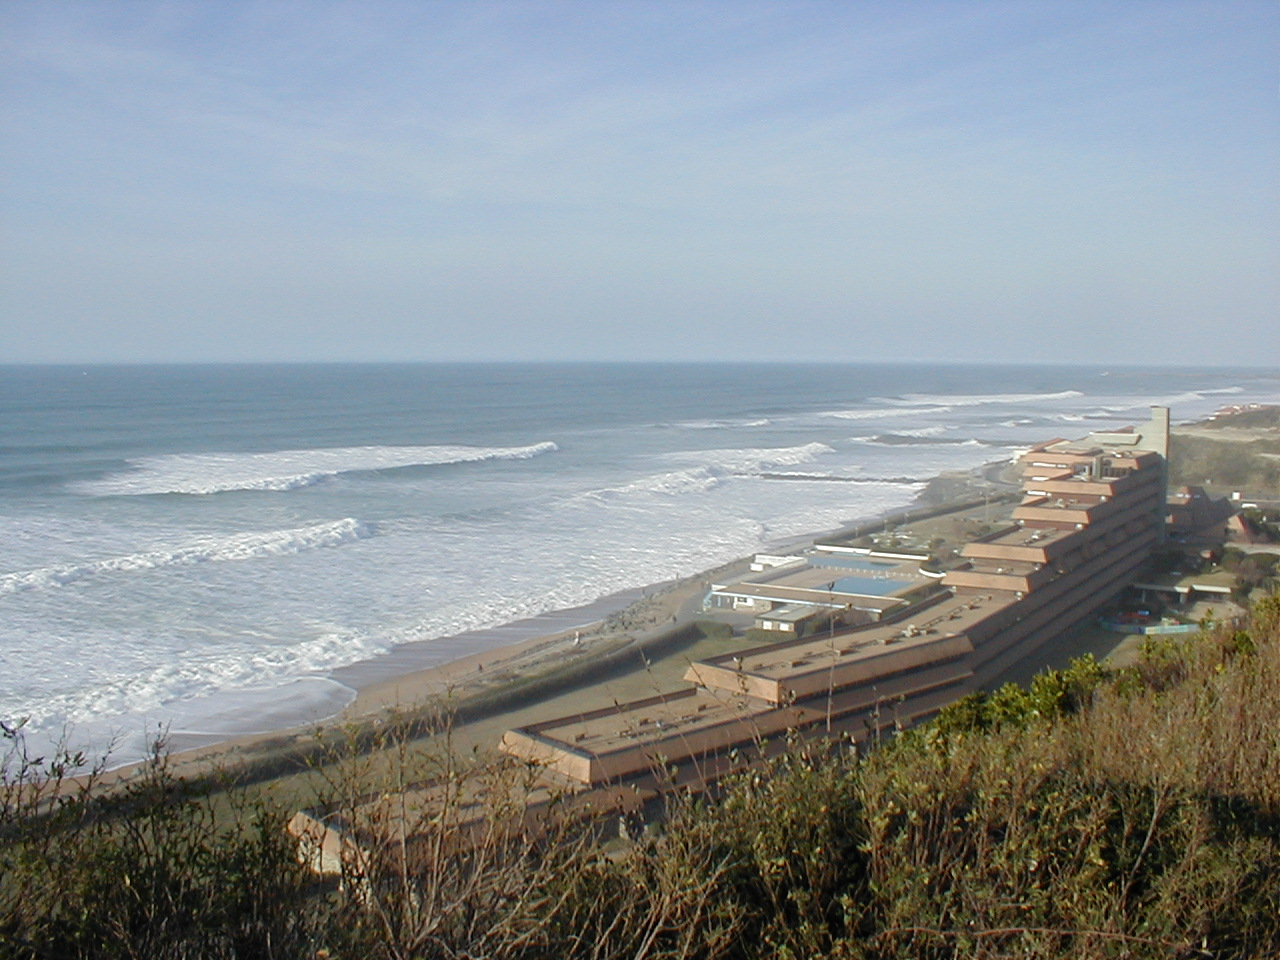
\includegraphics[width=.8\linewidth]{jfla.jpg}
  \caption{Les JFLA 2002, photographie par Maxence Guesdon}
  \label{fig:bienbelle}
\end{figure}

L'usage de~\texttt{includegraphics} avec une option~\texttt{width} permet une
utilisation facile d'images, comme illustré par la figure~\ref{fig:bienbelle}.

\subsection{Mathématiques}

Les environnements suivants ont été prédéfinis via le paquet~\texttt{amsthm}.

\begin{center}
  \begin{tabular}{lll}
    Environnement & Nom français & Nom anglais
    \\
    \hline
    \texttt{theo} & Théorème & \emph{Theorem}
    \\
    \texttt{prop} & Proposition & \emph{Proposition}
    \\
    \texttt{conj} & Conjecture & \emph{Conjecture}
    \\
    \texttt{coro} & Corollaire & \emph{Corollary}
    \\
    \texttt{lemm} & Lemme & \emph{Lemma}
    \\
    \texttt{defi} & Définition & \emph{Definition}
    \\
    \texttt{rema} & Remarque & \emph{Remark}
    \\
    \texttt{exem} & Exemple & \emph{Example}
  \end{tabular}
\end{center}

\subsection{Code source}

La classe~\texttt{jflart.cls} ne propose pas de paquet pour la coloration
syntaxique par défaut.
%
Les paquets~\texttt{listings} et~\texttt{minted} sont les plus fréquemment
utilisés.

\subsection{Bibliographie}

Vous pouvez au choix utiliser bibtex ou biblatex pour gérer votre bibliographie.
%
Merci d'utiliser le style de citation~\texttt{alpha-fr} avec bibtex, ou son
équivalent biblatex.

\subsection{Remerciements}

La classe ne propose pas d'environnement dédié pour les remerciements et sources de financement éventuelles.
%
Nous vous suggérons d'utiliser la commande~\cmd{paragraph\{Remerciements.\}} en
fin d'article.

\subsection{Autres ressources}

La classe~\texttt{jflart.cls} et sa documentation sont disponibles en
ligne~\cite{JFLART}.

\bibliographystyle{alpha-fr}
\bibliography{bibliography}

\end{document}
